\clearpage
\section{M-QAM Transmission System}

\begin{tcolorbox}	
	\begin{tabular}{p{2.75cm} p{0.2cm} p{10.5cm}} 	
		\textbf{Student Name}  & & Ana Luisa Carvalho (2017/04/01 - 2017/12/31) \\
                               & & Andoni Santos (2018/01/03 - )\\
		\textbf{Goal}          &:& M-QAM system implementation with BER measurement and comparison with theoretical and experimental values.\\
		\textbf{Directory} &:& sdf/m\_qam\_system
	\end{tabular}
\end{tcolorbox}

The goal of this project is to simulate a Quadrature Amplitude Modulation transmission system with M points in the constellation diagram (M-QAM) and to perform a Bit Error Rate (BER) measurement that can be compared with theoretical values.

%TODO: Verify
M-QAM systems can encode $\log_2 M$ bits per symbol which means they can transmit higher data rates keeping the same bandwidth when compared, for example, to PSK systems. However, because the states are closer together, these systems can be more susceptible to noise.

The Bit Error Rate (BER) is a measurement of how a bit stream is altered by a transmission system due to noise (among other factors). To study this effect we introduced Additive White Gaussian Noise (AWGN) to model thermal noise at the receiver.

For $M=4$ the M-QAM system reduces to a Quadrature Phase Shift Keying system (QPSK) system that uses four equispaced points in the constellation diagram (see figure \ref{fig:const}). Both these systems are also equivalent to the sum of two independent Binary Phase Shift Keying (BPSK) signals impressed on quadrature carriers.

\begin{figure}[h]
	\centering
	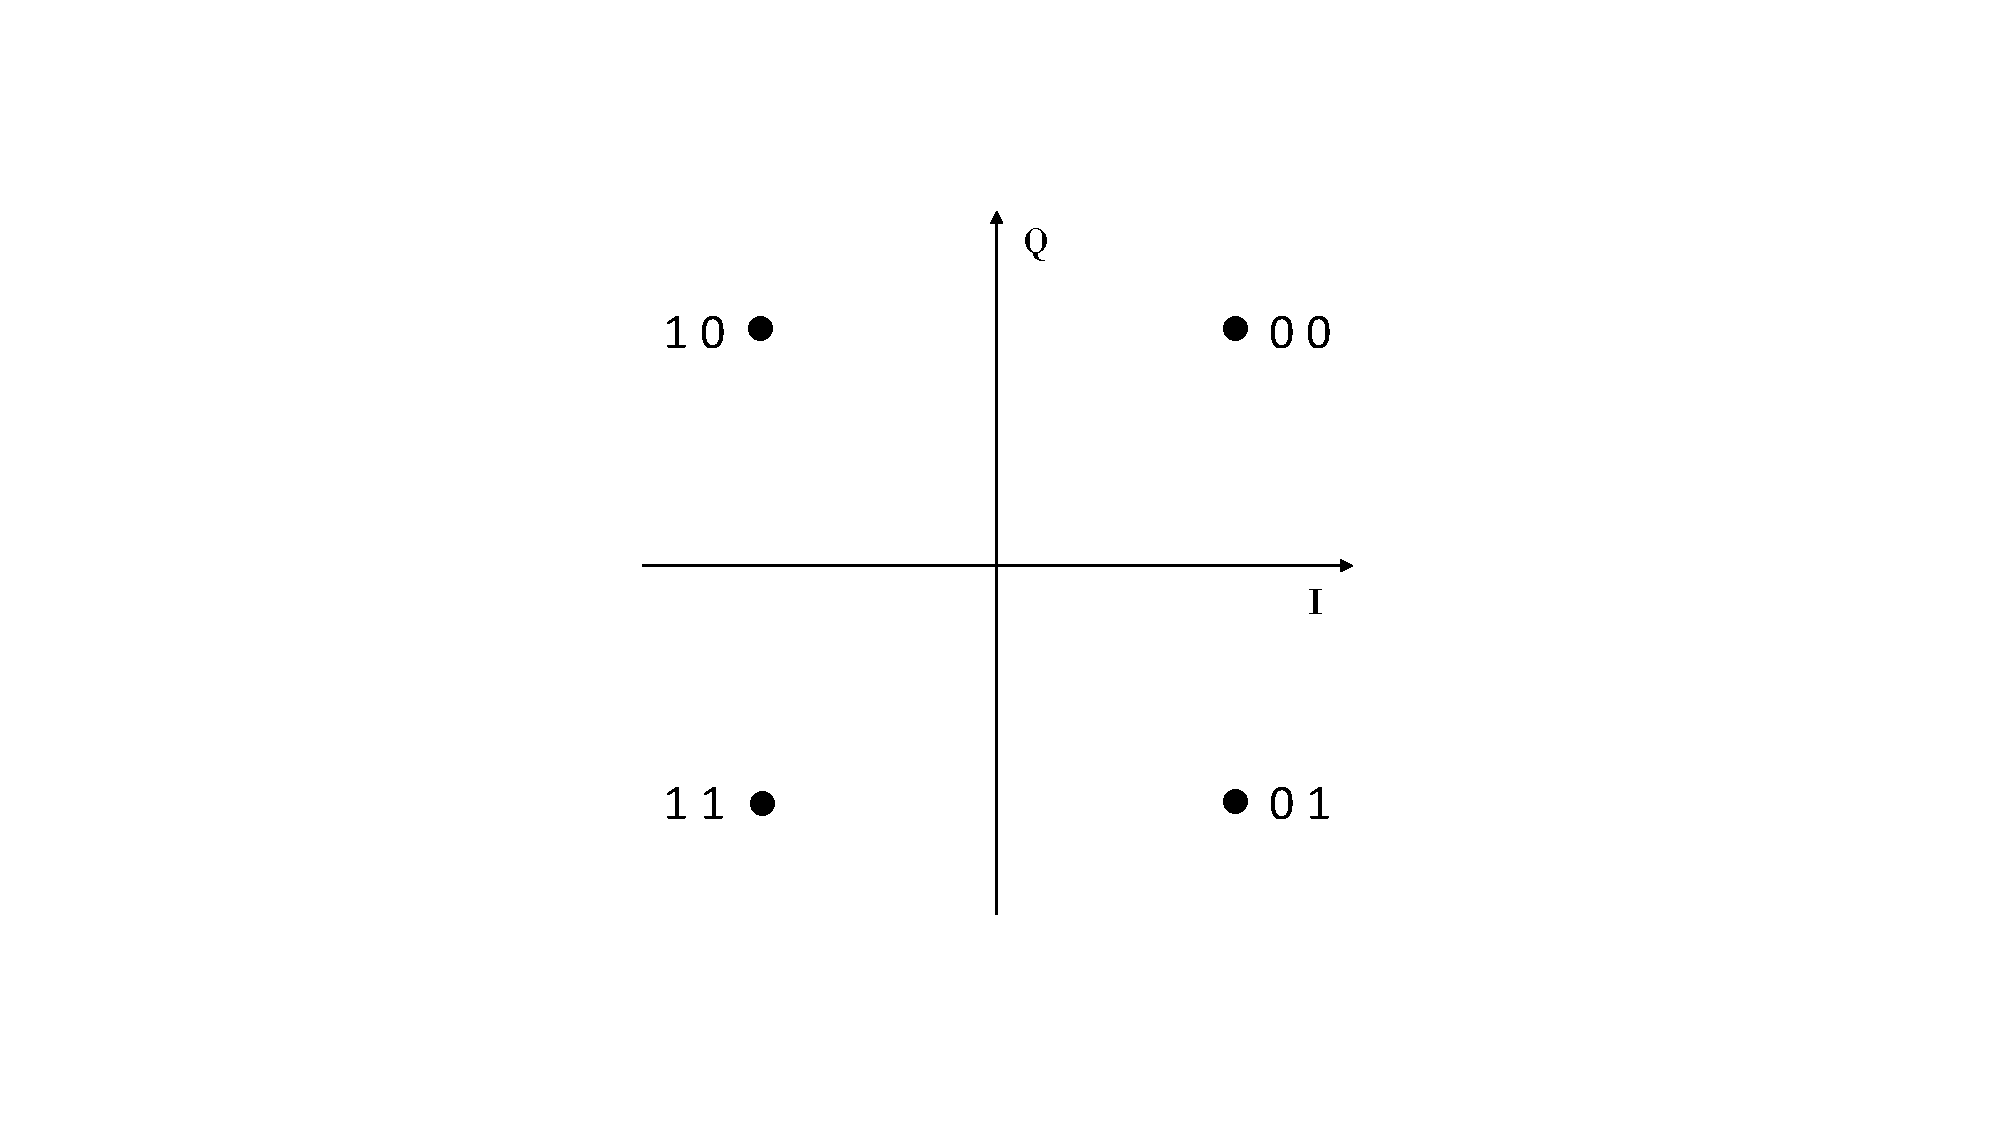
\includegraphics[clip, trim=1cm 3cm 1cm 3cm, width=\textwidth]{./sdf/m_qam_system/figures/MQAM_constellation.pdf}
	\caption{4-QAM constellation points.}
	\label{fig:const}
\end{figure}

%M can take several values: $2, 4, 16, 32, ...$. The first two correspond to BPSK and QPSK modulation, respectively.

\subsection{Theoretical Analysis}

M-QAM is a modulation scheme that takes advantage of two carriers (usually sinusoidal waves) with a phase difference of $\pi/2$. The resultant output consists of a signal with both amplitude and phase variations. The two carriers, referred to as I (In-phase) and Q (Quadrature), can be represented as

\begin{align}
	I=A\cos(\phi) \\
	Q=A\sin(\phi)
\end{align}
which means that any sinusoidal wave can be decomposed in its I and Q components:

\begin{align}
	A\cos(\omega~t+\phi)&=A\left(\cos(\omega~t)\cos(\phi)-\sin(\omega~t)\sin(\phi)\right) \\
	&=I\cos(\omega~t)-Q\sin(\omega~t),
\end{align}
where we have used the expression for the cosine of a sum and the definitions of I and Q.

%When demodulating a signal it is necessary to associate the received signal to the corresponding signal. The existence of noise in the channel means that we can only compute the probability that a given signal corresponds to a certain carrier and that's why we need to define the BER. Using
%
%\begin{equation}
%P_i f(s|c_i)>P_j f(s|c_j), \qquad i\neq j
%\end{equation}
%where $f(s|c_i)$ stands for the probability of detecting the signal $s$ given that $c_i$ was emmited. This inequallity can be rewritten in the following way
%
%\begin{equation}
%P(c_i|s)>P(c_j|s)
%\end{equation}
%where $P(c_i|s)$ and $P(c_j|s)$ are called \textit{a posteriori} probabilities and represent the probability that $c_i$ or $c_j$ were transmitted given that $s$ was received. In terms of the systems this simply means that we should select the signal most likely to have been transmitted.
%
%In the case of additive white gaussian noise the $f$ function is simply given by
%
%\begin{equation}
%f(s|c_i)=\frac{e^{-x^2/n_0}}{(\pi n_0)^{N/2}}
%\end{equation}
%where $x$ is the Euclidean distance in the I-Q plane between the signal received and carrier i and $N$ is the number of noise samples.
%
%When using 4-QAM modulation all points are at an equal distance from the origin (in the I-Q plane) so they all have the same energy given by
%
%\begin{equation}
%E=\frac{d^2}{2}
%\end{equation}
%where $d$ is the side of the square formed bye the constellation points.
%
%The probability that a given signal is identified correctly is given by
%
%\begin{equation}
%P_c=r^2
%\end{equation}
%where $n_0/2$ is the noise variance for AWGN and
%
%\begin{equation}
%r=\int_{-d/2}^{\infty}\frac{e^{-x^2/n_0}}{\sqrt{\pi n_0}} dx.
%\end{equation}
%
%The error probability, $P_e$, given by $1-P_c$ is given by
%
%\begin{equation}
%P_e=\erfc \sqrt{\frac{E}{2 n_0}}.
%\end{equation}

For the particular case of $M=4$, considering there is no crosstalk or interference between the Q and I components, the signal can be treated as a pair of independent BPSK systems.
Using Gray coding, adjacent symbols differ by only one bit. As such, an error in a single component leads to a single bit error.
This means that the probability of an error in bit detection is independent among components, as there is no crosstalk or interference. That being the case, the bit error rate can be exactly described by the same equation as in BPSK

%\begin{equation}
%P_b= Q\left(\sqrt{\frac{E_b}{n_0}}\right) = \frac{1}{2} erfc\left(\sqrt{\frac{E_b}{2 n_0}}\right).
%\end{equation}

%\begin{equation}\label{eq:berBPSK}
%P_{BE}= Q\left({\sqrt{\frac{2 E_b}{N_0}}}\right) = \frac{1}{2} \text{erfc}\left({\sqrt{\frac{ E_b}{N_0}}}\right).
%\end{equation}

%\begin{equation}\label{eq:berBPSK}
%BER= Q\left({G_{ele}\sqrt{\frac{2 P_L P_S}{n_0}}}\right) = \frac{1}{2} \text{erfc}\left({G_{ele}\sqrt{\frac{P_L P_S}{n_0}}}\right).
%\end{equation}

\begin{equation}\label{eq:berBPSK}
P_b= Q\left({\frac{m}{n_0}}\right) = \frac{1}{2} \text{erfc}\left({\frac{m}{N_0}}\right).
\end{equation}

with


\begin{eqnarray}
&m &= G_{ele} \sqrt{P_L P_S} \\
&N_0 &= \sqrt{2 n_0}
\end{eqnarray}
%\begin{equation}\label{eq:berBPSK}
%BER= Q\left({G_{ele}\sqrt{\frac{2 P_L P_S}{n_0}}}\right) = \frac{1}{2} \text{erfc}\left({G_{ele}\sqrt{\frac{P_L P_S}{n_0}}}\right).
%\end{equation}

where $P_L$ is the local oscillator power, $P_S$ is the optical signal power, $G_{ele}$ is the gain in the transimpedance amplifier and $n_0$ is the noise spectral density.

The symbol error rate however is not the same, as it depends on both bits being correctly detected. The probability of both bits being correctly detected is:

\begin{equation}
P_C = (1 - P_b)^2
\end{equation}

From this, the probability of symbol error is:

\begin{eqnarray}
&P_s &= 1-P_C =\nonumber \\
&	   &= 1 - \left(1 - Q \left({\frac{m \sqrt{2}}{n_0}}\right)\right)^2 = \nonumber \\
&	   &= 2 Q\left({\frac{m \sqrt{2}}{n_0}}\right)\left[1-\frac{1}{2} Q \left({\frac{\sqrt{2} m}{n_0}}\right)\right]
\end{eqnarray}

%The bit error rate is then equal to the probability of the phase falling outside the correct detection range in a given component due to noise,


%Exact solutions for the probability of symbol and bit errors exist only for $M=4$.

%As previously mentioned, for $M=4$ the system is reduced to a QPSK system. Knowing that the AWGN is independent

%For the cases of $M>4$, an aproximation can be used.
%The probability of symbol error, $P_s$, in coherent M-PSK demodulation with AWGN can be aproximated by
%
%\begin{equation}
%	P_s=2~Q\left(\sqrt{2~\log_2 M \left(\frac{E_b}{n_0}\right)\sin^2\frac{\pi}{M}}\right)
%\end{equation}
%where $E_b$ is the energy of one bit, $n_0$ is the noise power and the function $Q$ is defined as
%\begin{equation}
%	Q(x)=\frac{1}{2} erfc\left(\frac{x}{\sqrt{2}}\right).
%	\label{eq:Ps}
%\end{equation}
%
%It is worth noting that this aproximation is only valid for high SNR values. The probability of bit errors for $M>4$ can now be estimated, as it is related to $P_s$ by
%
%\begin{equation}
%	P_b=\frac{1}{\log_2 M}P_s.
%	\label{eq:Pb}
%\end{equation}
%
%For QPSK we get, using $M=4$ in equations \ref{eq:Ps} and \ref{eq:Pb},
%\begin{equation}
%	P_b= 2 Q\left(\sqrt{\frac{2~E_b}{n_0}}\right) = erfc\left(\sqrt{\frac{E_b}{n_0}}\right).
%\end{equation}
%
%The exact probability bit error for $M=4$ are

%The Bit Error Rate curve given by~\eqref{eq:berBPSK} is plotted in figure \ref{fig:QPSK_th_curve} as a function of the optical signal power for $N_0=10^{-6}$, $P_L = 0~dBm$ and $G_{ele} = 10^3$.

%\begin{figure}[h]
%		\centering
%		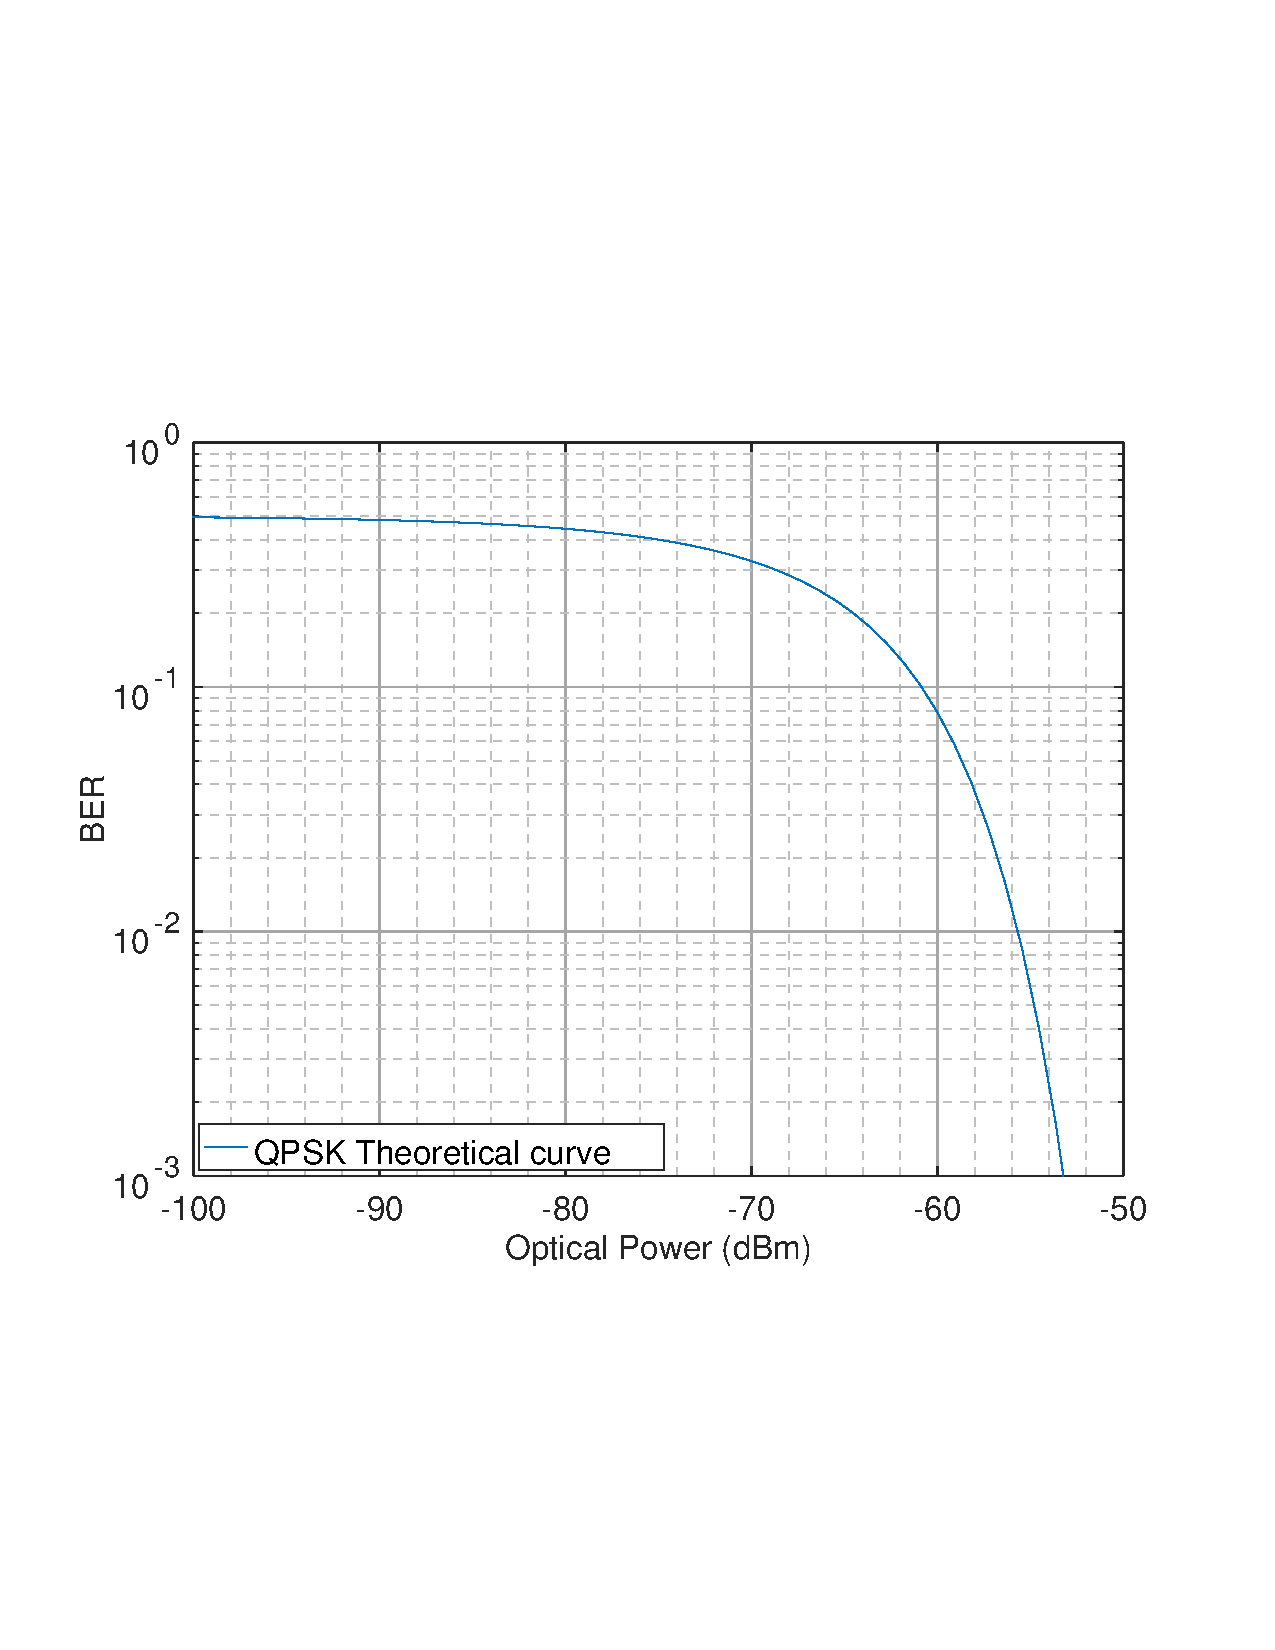
\includegraphics[clip, trim=2cm 6cm 2cm 6cm, width=0.7\textwidth]{./sdf/m_qam_system/figures/BER_QPSK_theory_20180119.pdf}
%		\caption{QPSK theoretical BER values as a function of the output optical power in dBm.}
%		\label{fig:QPSK_th_curve}
%\end{figure}

It's worth noting that these equations are only valid for M=4, as in that case the system is similar to QPSK with a 4 point constellation. For $M > 4$ a different approach is required.

It is possible to further decrease the error rate by using a matched filter before sampling the signal. In this case, the resulting signal will still have gaussian noise, but the SNR will be greatly improved. This can be achieved, for instance by using a root-raised cosine filter at the pulse shaper and another one before the sampler. Intersymbol interference will still be minimal as it is equivalent to a raised cosine filter, where half the filtering is done on the transmitter side (while pulse-shaping) and the other half is done on the receiver side, before sampling.


The optimal BER that can be obtained by using matched filtering is described by~\cite{mischasch}:

\begin{equation}\label{eq:berBPSK}
P_b= \frac{1}{2} \text{erfc}\left({\frac{m_{mf}}{N_{mf}}}\right)
\end{equation}

with

\begin{eqnarray}
&m_{mf} &= \frac{1}{2} T G_{ele} \sqrt{P_L P_S} \\
&N_{mf} &= \sqrt{\frac{T n_0}{4}}
\end{eqnarray}


Figure~\ref{fig:QPSK_th_curves} show the curves for both these equations, in the case where  $n_0=10^{-6}$, $P_L = 0~dBm$ and $G_{ele} = 10^3$.
%Here, $T$ is the symbol period. 

\begin{figure}[h]
		\centering
		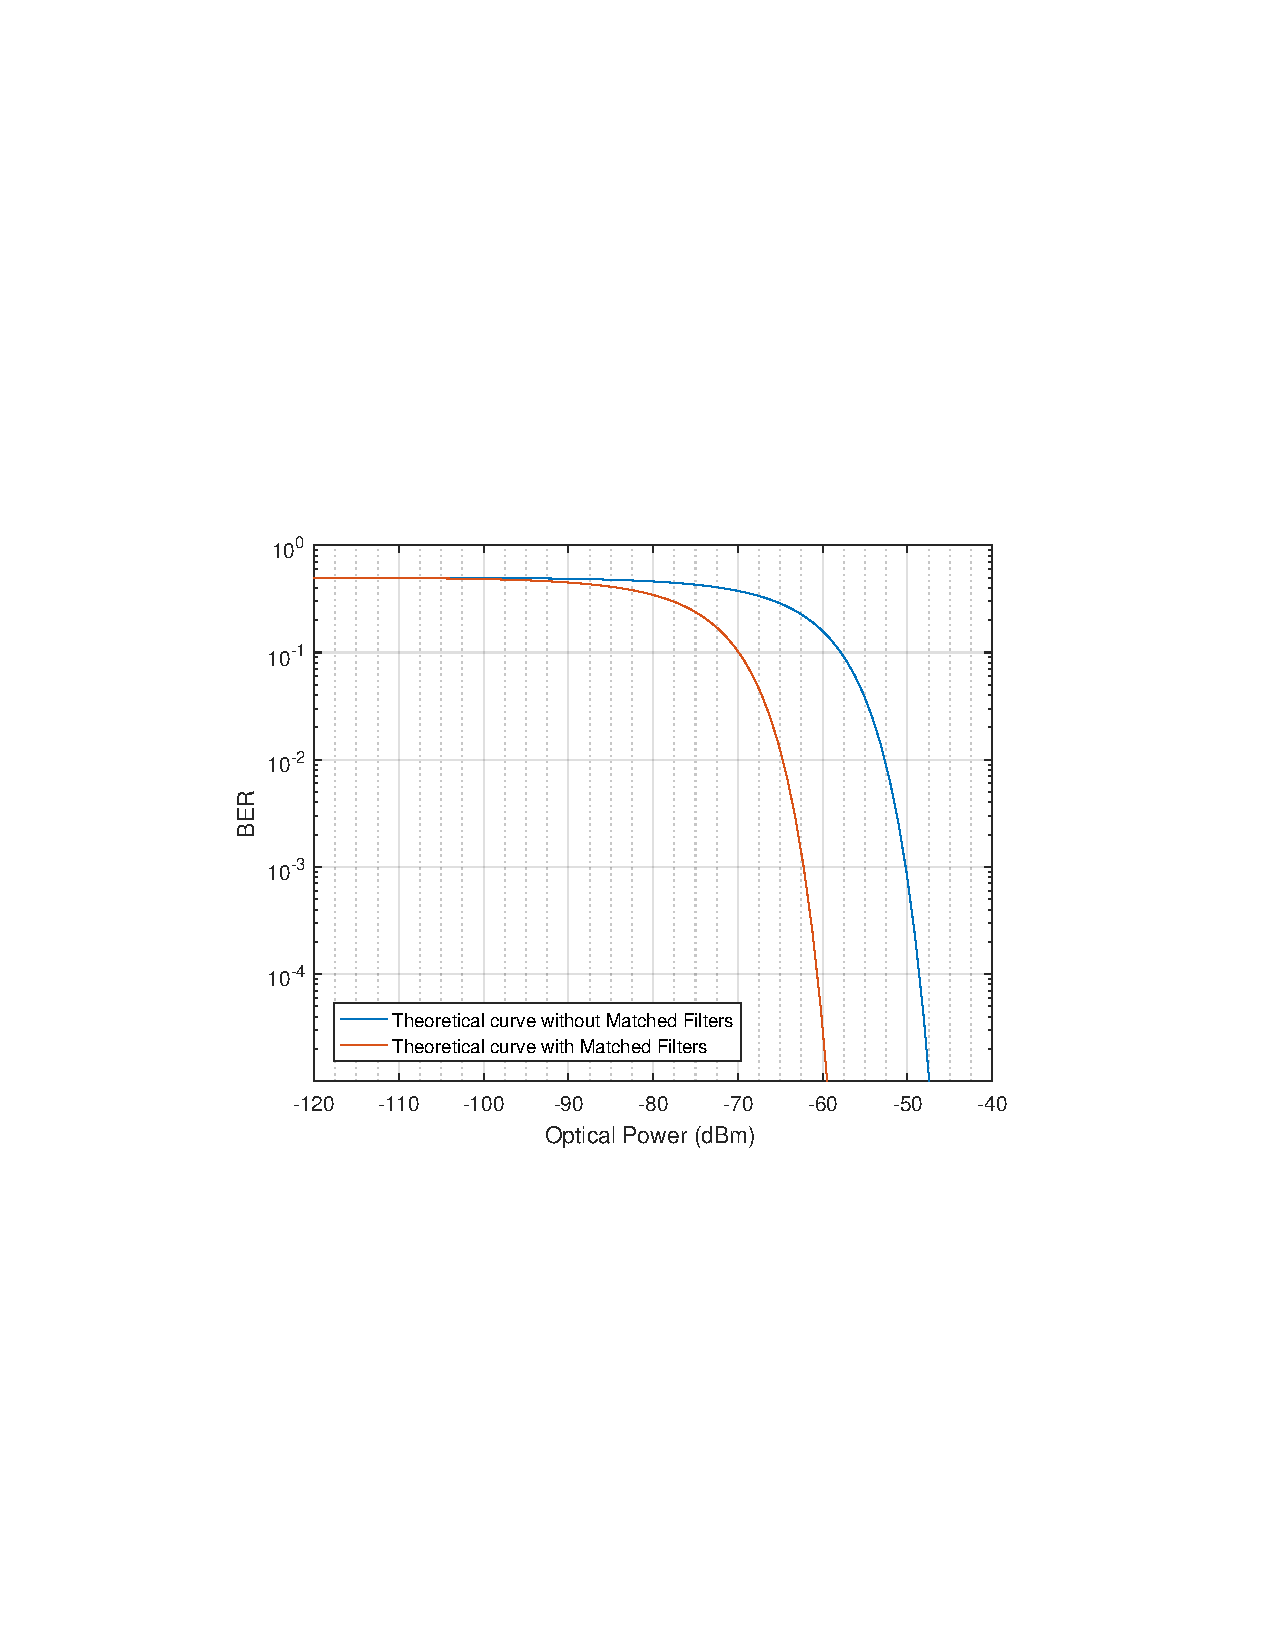
\includegraphics[clip, trim=4cm 8cm 4cm 8cm, width=0.7\textwidth]{./sdf/m_qam_system/figures/teor_BER_curves.pdf}
		\caption{QPSK theoretical BER values as a function of the output optical power in dBm.\label{fig:QPSK_th_curves}}	
\end{figure}

% TODO: preencher isto depois de requisitar o livro


\subsection{Simulation Analysis}

\begin{figure}[h]
	\centering
	
\includegraphics[width=0.8\textwidth]{./sdf/m_qam_system/figures/simulation_mqam}
	\caption{Schematic representation of the MQAM system.}\label{MQAM_system_block_diagram}
\end{figure}

The M-QAM transmission system is a complex block of code that simulates the modulation, transmission and
demodulation of an optical signal using M-QAM modulation.
It is composed of four blocks: a transmitter, a receiver, a sink and a block that performs a Bit Error Rate (BER) measurement. The schematic representation of the
system is presented in figure \ref{MQAM_system_block_diagram}.
	
\paragraph{Current state:} The system currently being implement is a QPSK system (M=4).

\paragraph{Future work:} Extend this block to include other values of M.

\subsection*{Functional description}

A complete description of the M-QAM transmitter and M-QAM homodyne receiver blocks can be found in the \textit{Library} chapter of this document as well as a detailed description of the independent blocks that compose these blocks.

The M-QAM transmitter generates one or two optical signals by encoding a binary string using M-QAM modulation. It also outputs a binary signal that is used to perform the BER measurement.

The M-QAM homodyne receiver accepts one input optical signal and outputs
a binary signal. It performs the M-QAM demodulation of the input signal by combining the optical signal with a local oscillator.

The demodulated optical signal is compared to the binary one produced by the transmitter in order to estimate the Bit Error Rate (BER).

The files used are summarized in tables~\ref{tab:sources} and~\ref{tab:headers}. These include all blocks and sub-blocks used and allow for the full operation of the M-QAM system.

\subsection*{Required files}\label{Required files}

\begin{table}[H]
    \centering
    \begin{tabulary}{1.0\textwidth}{|p{7.5cm}|p{5.5cm}|p{1cm}|}
        \hline
        \multicolumn{3}{|c|}{ \textbf{Source Files} } \\
        \hline
        \textbf{File}                      			 & \textbf{Comments} & \textbf{Status} \\ \hline
        add\_20171116.cpp                            &                   & \checkmark \\ \hline
        binary\_source\_20180118.cpp                 &                   & \checkmark \\ \hline
        bit\_error\_rate\_20171810.cpp               &                   & \checkmark \\ \hline
        decoder\_20180118.cpp                        &                   & \checkmark \\ \hline
        discrete\_to\_continuous\_time\_20180118.cpp &                   & \checkmark \\ \hline
        homodyne\_receiver\_20180118.cpp             & $^{1}$			 & \checkmark \\ \hline
        ideal\_amplififer\_20180118.cpp              &                   & \checkmark \\ \hline
        iq\_modulator\_20180118.cpp                  &                   & \checkmark \\ \hline
        local\_oscillator\_20180118.cpp              &                   & \checkmark \\ \hline
        m\_qam\_mapper\_20180118.cpp                 &                   & \checkmark \\ \hline
        m\_qam\_system.cpp                 			 & $^{2}$   		 & \checkmark \\ \hline
        m\_qam\_transmitter\_20180118.cpp            &                   & \checkmark \\ \hline
        netxpto\_20180118.cpp                        & $^{2}$ 			 & \checkmark \\ \hline
        optical\_hybrid\_20180118.cpp                &                   & \checkmark \\ \hline
        photodiode\_old\_20180118.cpp                &                   & \checkmark \\ \hline
        pulse\_shaper\_20180118.cpp                  &                   & \checkmark \\ \hline
        sampler\_20171119.cpp                        &                   & \checkmark \\ \hline
        sink\_20180118.cpp                           &                   & \checkmark \\ \hline
        super\_block\_interface\_20180118.cpp        & $^{2}$ 			 & \checkmark \\ \hline
        white\_noise\_20180118.cpp                   & 					 & \checkmark \\ \hline
    \end{tabulary}

    \caption{$^1$ The library entry is under a different name, \textit{m\_qam\_receiver};\\
    $^2$ No library entry as it is a main or general purpose file, not a specific block. 	 \label{tab:sources}}
\end{table}

\begin{table}[H]
    \centering
    \begin{tabulary}{1.0\textwidth}{|p{7cm}|p{6cm}|p{1cm}|}
        \hline
        \multicolumn{3}{|c|}{ \textbf{Header Files} } \\
        \hline
        \textbf{File}                      & \textbf{Comments} & \textbf{Status} \\ \hline
        add\_20180118.h                            & $^{1}$			   & \checkmark \\ \hline
        binary\_source\_20180118 .h                &                   & \checkmark \\ \hline
        bit\_error\_rate\_20171810.h               & $^{1}$            & \checkmark \\ \hline
        decoder\_20180118.h                        &                   & \checkmark \\ \hline
        discrete\_to\_continuous\_time\_20180118.h &                   & \checkmark \\ \hline
        homodyne\_receiver\_20171203.h             & $^{1,2}$          & \checkmark \\ \hline
        ideal\_amplifier\_20180118.h               &                   & \checkmark \\ \hline
        iq\_modulator\_20180118.h                  &                   & \checkmark \\ \hline
        local\_oscillator\_20180118.h              &                   & \checkmark \\ \hline
        m\_qam\_mapper\_20180118.h                 &                   & \checkmark \\ \hline
        m\_qam\_transmitter\_20180118.h            &                   & \checkmark \\ \hline
        netxpto\_20180118.h                        & $^3$ 			   & \checkmark \\ \hline
        optical\_hybrid\_20180118.h                &                   & \checkmark \\ \hline
        photodiode\_old\_20180118.h                &                   & \checkmark \\ \hline
        pulse\_shaper\_20180118.h                  &                   & \checkmark \\ \hline
        sampler\_20171119.h                        & $^1$              & \checkmark \\ \hline
        sink\_20180118.h                           &                   & \checkmark \\ \hline
        super\_block\_interface\_20180118.h        & $^3$			   & \checkmark \\ \hline
        white\_noise\_20180118.h                   &                   & \checkmark \\ \hline
    \end{tabulary}
    \caption{$^1$ This file does not share the same time-tag as the corresponding ".cpp" file.\\$^2$ The library entry is under a different name, \textit{m\_qam\_receiver}\\
    $^3$ No library entry as it is a main or general purpose file, not a specific block. \label{tab:headers}}
\end{table}

%\begin{table}[]
%	\centering
%	\caption{Main system files}
%	\begin{tabular}{|c|c|c|c|ccc}
%		\cline{1-4}
%		\textbf{System blocks} & \textbf{Source file} & \textbf{Header file}  &  \textbf{Status} & \\ \cline{1-4}
%		Main & m\_qam\_system\_sdf.cpp & --- & \checkmark & \\ \cline{1-4}
%		M-QAM transmitter & m\_qam\_transmitter\_20180118.cpp & m\_qam\_transmitter\_20180118.h & \checkmark &  \\ \cline{1-4}
%		M-QAM receiver & homodyne\_receiver\_20180118.cpp & homodyne\_receiver\_20180118.h & \checkmark &  \\ \cline{1-4}
%		Sink & sink\_20180118.cpp & sink\_20180118.h &  \checkmark & \\ \cline{1-4}
%		BER estimator & bit\_error\_rate\_20171810.cpp & bit\_error\_rate\_20171810.h & \checkmark &\\ \cline{1-4}
%	\end{tabular}
%	\label{files_table}
%\end{table}

%\subsection*{Required Files}
%
%The required header and source files needed to run this system are summarized in table \ref{table:files}.
%
%\begin{table}
% 	\centering
% 	\caption{Required files}
% 	\begin{tabular}{|c|c|p{40mm}|c|ccp{40mm}c}
% 		\cline{1-4}
% 		\textbf{Header file} & \textbf{Source file} & \textbf{Description} &  \textbf{Status} & \\ \cline{1-4}
% 		add.h & add.cpp & Adds two signals.  & \checkmark &   \\ \cline{1-4}
% 		binary\_source.h & binary\_source.cpp & Produces a binary sequence. & \checkmark & \\ \cline{1-4}
% 		bit\_error\_rate.h & bit\_error\_rate.cpp & Computes the BER and writes it to a text file. & \checkmark & \\ \cline{1-4}
% 		discrete\_to\_continuous\_time.h & discrete\_to\_continuous\_time.cpp & Converts a signal from discrete in time to continuous in time. & \checkmark & \\ \cline{1-4}
% 		homodyne\_receiver.h & m\_qam\_homodyne\_receiver.cpp & & \\ \cline{1-4}
% 		ideal\_amplifier.h & ideal\_amplifier.cpp & Amplifies the signal. & \checkmark & \\ \cline{1-4}
% 		iq\_modulator.h & iq\_modulator.cpp & Divides the signal in its quadrature and in phase components & \checkmark &\\ \cline{1-4}
% 		local\_oscillator.h & local\_oscillator.cpp & & & \checkmark &\\ \cline{1-4}
% 		m\_qam\_mapper.h & m\_qam\_mapper.cpp & Maps the signal using the defined constellation & \checkmark & \\ \cline{1-4}
% 		m\_qam\_transmitter.h & m\_qam\_transmitter.cpp & & \checkmark & \\ \cline{1-4}
% 		netxpto.h & netxpto.cpp & General class that contains definition from signals and buffers. & \checkmark &\\ \cline{1-4}
% 		optical\_hybrid.h & optical\_hybrid.cpp & Implements an optical hybrid. & \checkmark & \\ \cline{1-4}
% 		photodiode\_old.h & photodiode\_old.cpp & Pair of photodiodes and current subtraction. & \checkmark & \\ \cline{1-4}
% 		pulse\_shaper.h & pulse\_shaper.cpp & Electrical filter. & \checkmark &\\ \cline{1-4}
% 		sampler\_20171119.h & sampler\_20171119.cpp & Samples the signal. & \checkmark &\\ \cline{1-4}
% 		sink.h & sink.cpp & Deletes signal. & \checkmark & \\ \cline{1-4}
% 		super\_block\_interface.h & super\_block\_interface.cpp & & \checkmark &\\ \cline{1-4}
% 		white\_noise.h & white\_noise.cpp & Generates white gaussian noise. & \checkmark &\\ \cline{1-4}
% 	\end{tabular}
% 	\label{table:files}
%\end{table}
\pagebreak
\subsection*{Input Parameters}

The system accepts several input parameters that can be defined by the user. These are described in table \ref{table:in_par}.

\begin{table}[H]
	\centering
	\caption{Input parameters}
	\begin{tabular}{|c|c|p{70mm}|ccp{70mm}}
		\cline{1-3}
		\textbf{Parameter} & \textbf{Type} & \textbf{Description} &    \\ \cline{1-3}
		numberOfBitsGenerated & t\_integer & Determines the number of bits to be generated by the binary source  &    \\ \cline{1-3}
		samplesPerSymbol & t\_integer & Number of samples per symbol &    \\ \cline{1-3}
		prbsPatternLength & int & Determines the length of the pseudorandom sequence pattern (used only when the binary source is operated in \textit{PseudoRandom} mode) &    \\ \cline{1-3}
		bitPeriod & t\_real & Temporal interval occupied by one bit &    \\ \cline{1-3}
		rollOffFactor\_shp & t\_real & Parameter of the pulse shaper filter &    \\ \cline{1-3}
		rollOffFactor\_out & t\_real & Parameter of the output filter &    \\ \cline{1-3}
		shaperFilter & enum & Type of filter used in Pulse Shaper &    \\ \cline{1-3}
		outputFilter & enum & Type of filter used in output filter &    \\ \cline{1-3}
		seedType & enum & Method of seeding noise generators &    \\ \cline{1-3}
		seedArray & array<int,2> & Seeds to initialize noise generators &    \\ \cline{1-3}
		signalOutputPower\_dBm & t\_real & Determines the power of the output optical signal in dBm &  \\ \cline{1-3}
		numberOfBitsReceived & int &   Determines when the simulation should stop. If $-1$ then it only stops when there is no more bits to be sent&   \\ \cline{1-3}
		iqAmplitudeValues & vector<t\_iqValues> & Determines the constellation used to encode the signal in IQ space &    \\ \cline{1-3}
		symbolPeriod & double & Given by bitPeriod/samplesPerSymbol &    \\ \cline{1-3}
		localOscillatorPower\_dBm & t\_real & Power of the local oscillator &    \\ \cline{1-3}
		responsivity & t\_real & Responsivity of the photodiodes (1 corresponds to having all optical power transformed into electrical current) &    \\ \cline{1-3}
		amplification & t\_real & Amplification provided by the ideal amplifier &    \\ \cline{1-3}
		noiseAmplitude & t\_real & Amplitude of the white noise &    \\ \cline{1-3}
		samplesToSkip & t\_integer & Number of samples to be skipped by the \textit{sampler} block &    \\ \cline{1-3}
		confidence & t\_real & Determines the confidence limits for the BER estimation &    \\ \cline{1-3}
		midReportSize & t\_integer &  &    \\ \cline{1-3}
		bufferLength & t\_integer & Corresponds to the number of samples that can be processed in each run of the system &    \\ \cline{1-3}
		\end{tabular}
		\label{table:in_par}
		\end{table}

\subsection*{Simulation results}

In this section we show the eye diagrams for the S1 signals for two different values of the output optical power.

\begin{figure}[h]
	\centering
	\begin{subfigure}{.5\textwidth}
		\centering
		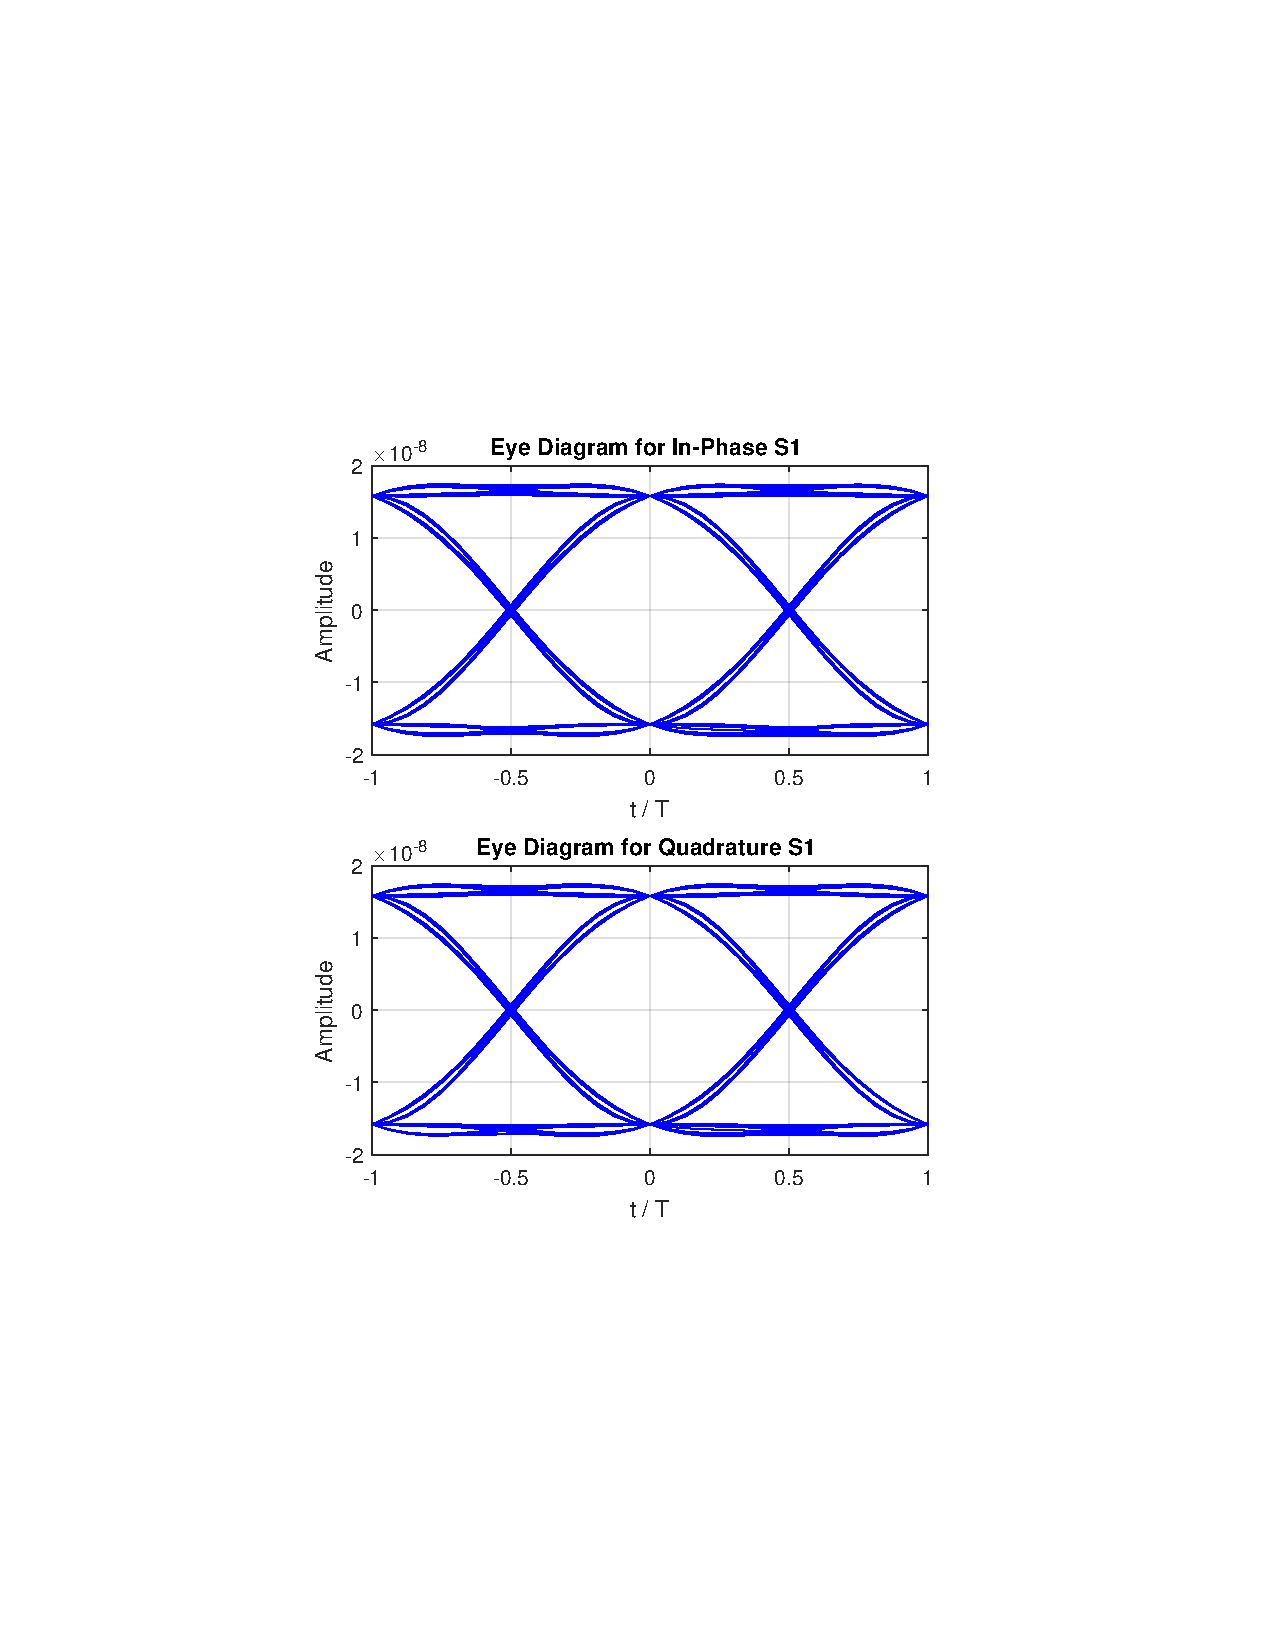
\includegraphics[clip, trim=5cm 7cm 5cm 7cm, width=\textwidth]{./sdf/m_qam_system/figures/eye120db09ro.pdf}
	\end{subfigure}%
	\begin{subfigure}{.5\textwidth}
		\centering
		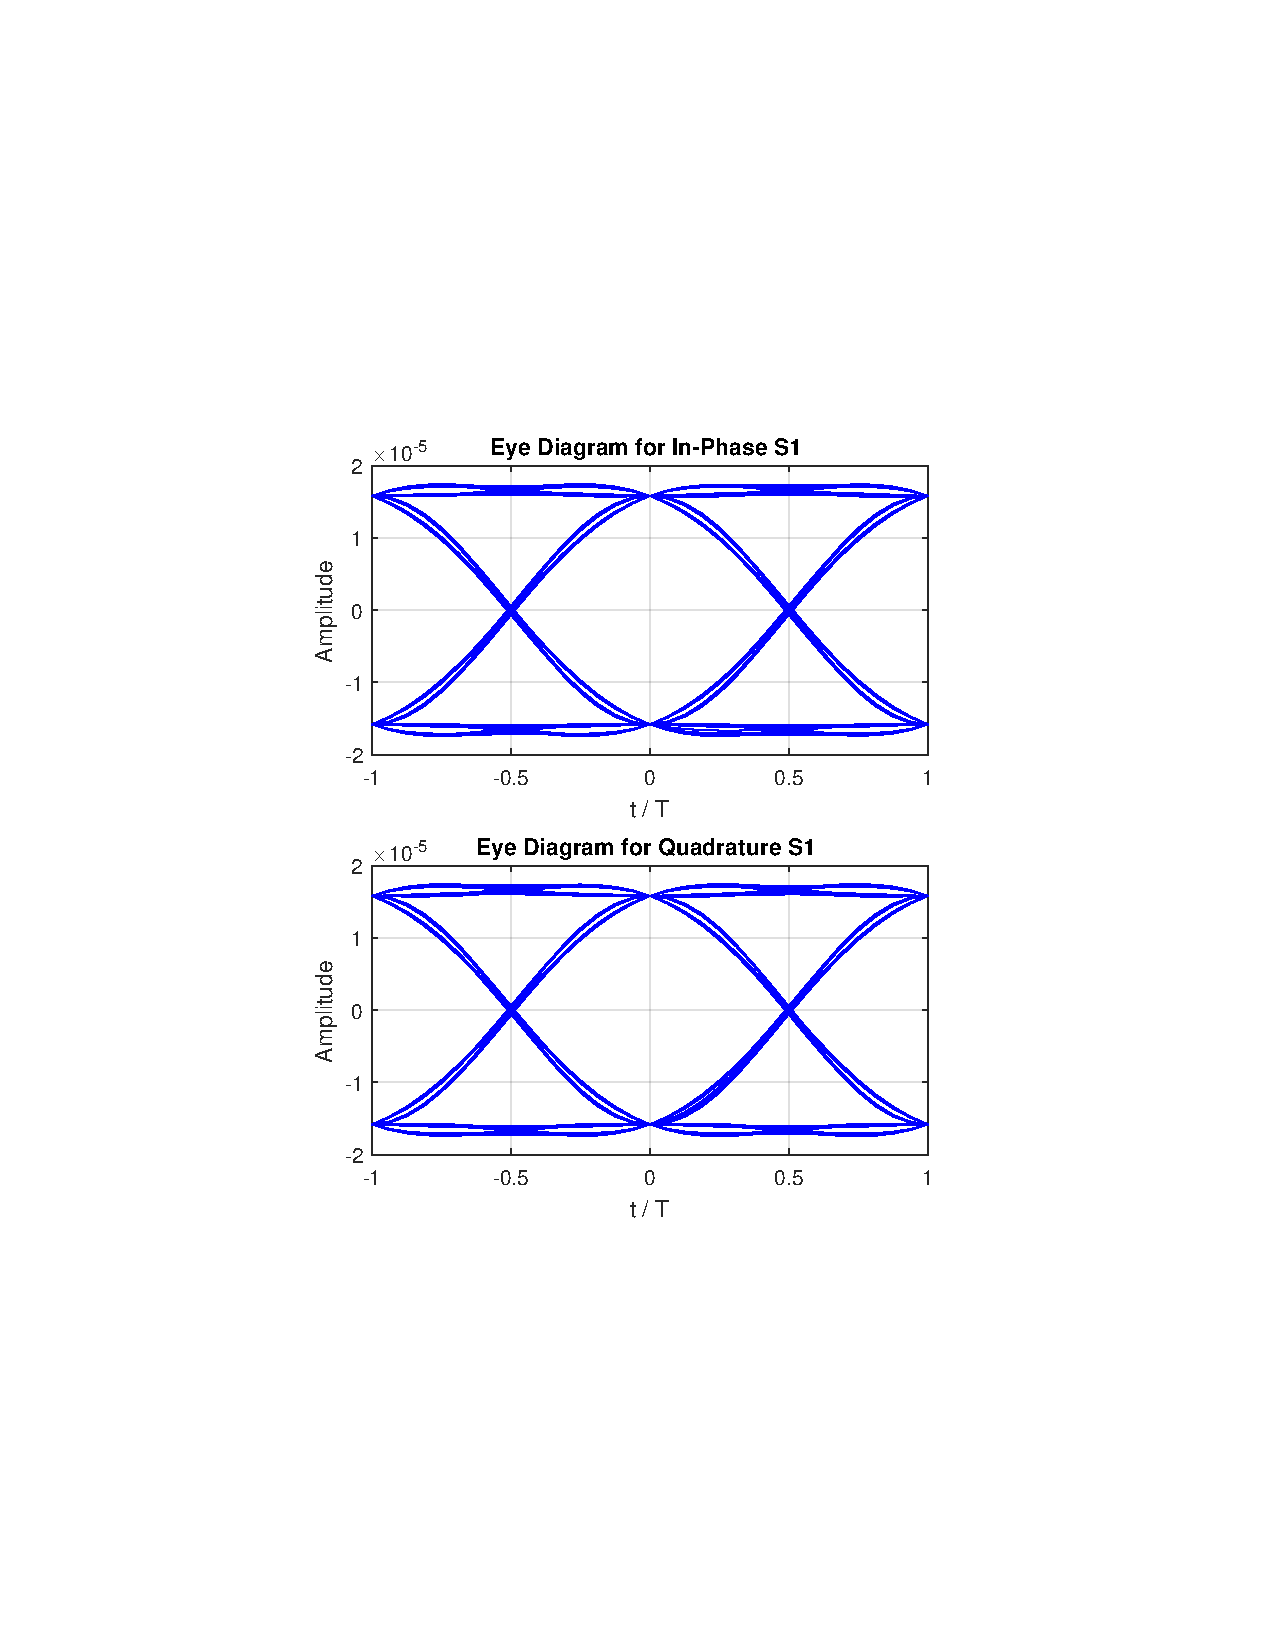
\includegraphics[clip, trim=5cm 7cm 5cm 7cm, width=\textwidth]{./sdf/m_qam_system/figures/eye60db09ro.pdf}
	\end{subfigure}
	\caption{Eye diagrams for the S1 bandpass signal with an output optical power of $-120$dBm (left) and $-60$dBm (right). Note different scales on y axis.}
	\label{fig:test}
\end{figure}

\subsection*{Experimental Analysis}
\begin{figure}[H]
	\centering
	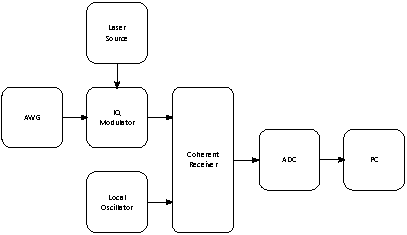
\includegraphics[width=0.8\textwidth]{./sdf/m_qam_system/figures/mqamExperimental20180206.pdf}
	\caption{Experimental setup}
	\label{fig:experimental_mqam_setup}
\end{figure}
%
%
\begin{table}[H]
	\centering
	\begin{tabulary}{1.0\textwidth}{|L|L|l|}
%		\hline
%		\textbf{Device}		& \textbf{Description}\\
%		\hline
%		Balanced Photodetector	& Thorlabs PDB 450C\\
%		\hline
%%		BS					& Beam Splitter\\
%		\hline
%%		Pulse Generator		& HP 8116A Pulse Generator\\
%		\hline
%%		Amplitude Modulator	& Mach Zehnder SDL OC 48\\
%		\hline
%%		VOA					& Eigenlicht Power Meter 420\\
%		\hline
%%		VOA					& Thorlabs VOA 45-APC\\
%%		\hline
%%		PIN					& Thorlabs PDB 450C\\
%		\hline
%%		ADC					& Picoscope 6403D\\
%		\hline
	\end{tabulary}
\end{table}


\subsection{Comparative Analysis}

In this section we show the simulation results and compared them with the theoretical predictions for an M-QAM system with $M=4$. Figure \ref{fig:ber_pseudorandom} shows the variation of the BER with the optical power of the signal, using $40000$ bits produced by a random number generator. The noise power was set at $10^{-6}$, the local oscillator at $0~dBm$ and the amplification at the transimpedance amplifier was set at $10^3$.
The blue line represents the theoretical curve, while the orange points represent the simulated values with the respective confidence margins. The simulation agrees closely with the theoretical values.

\begin{figure}[h]
	\centering
	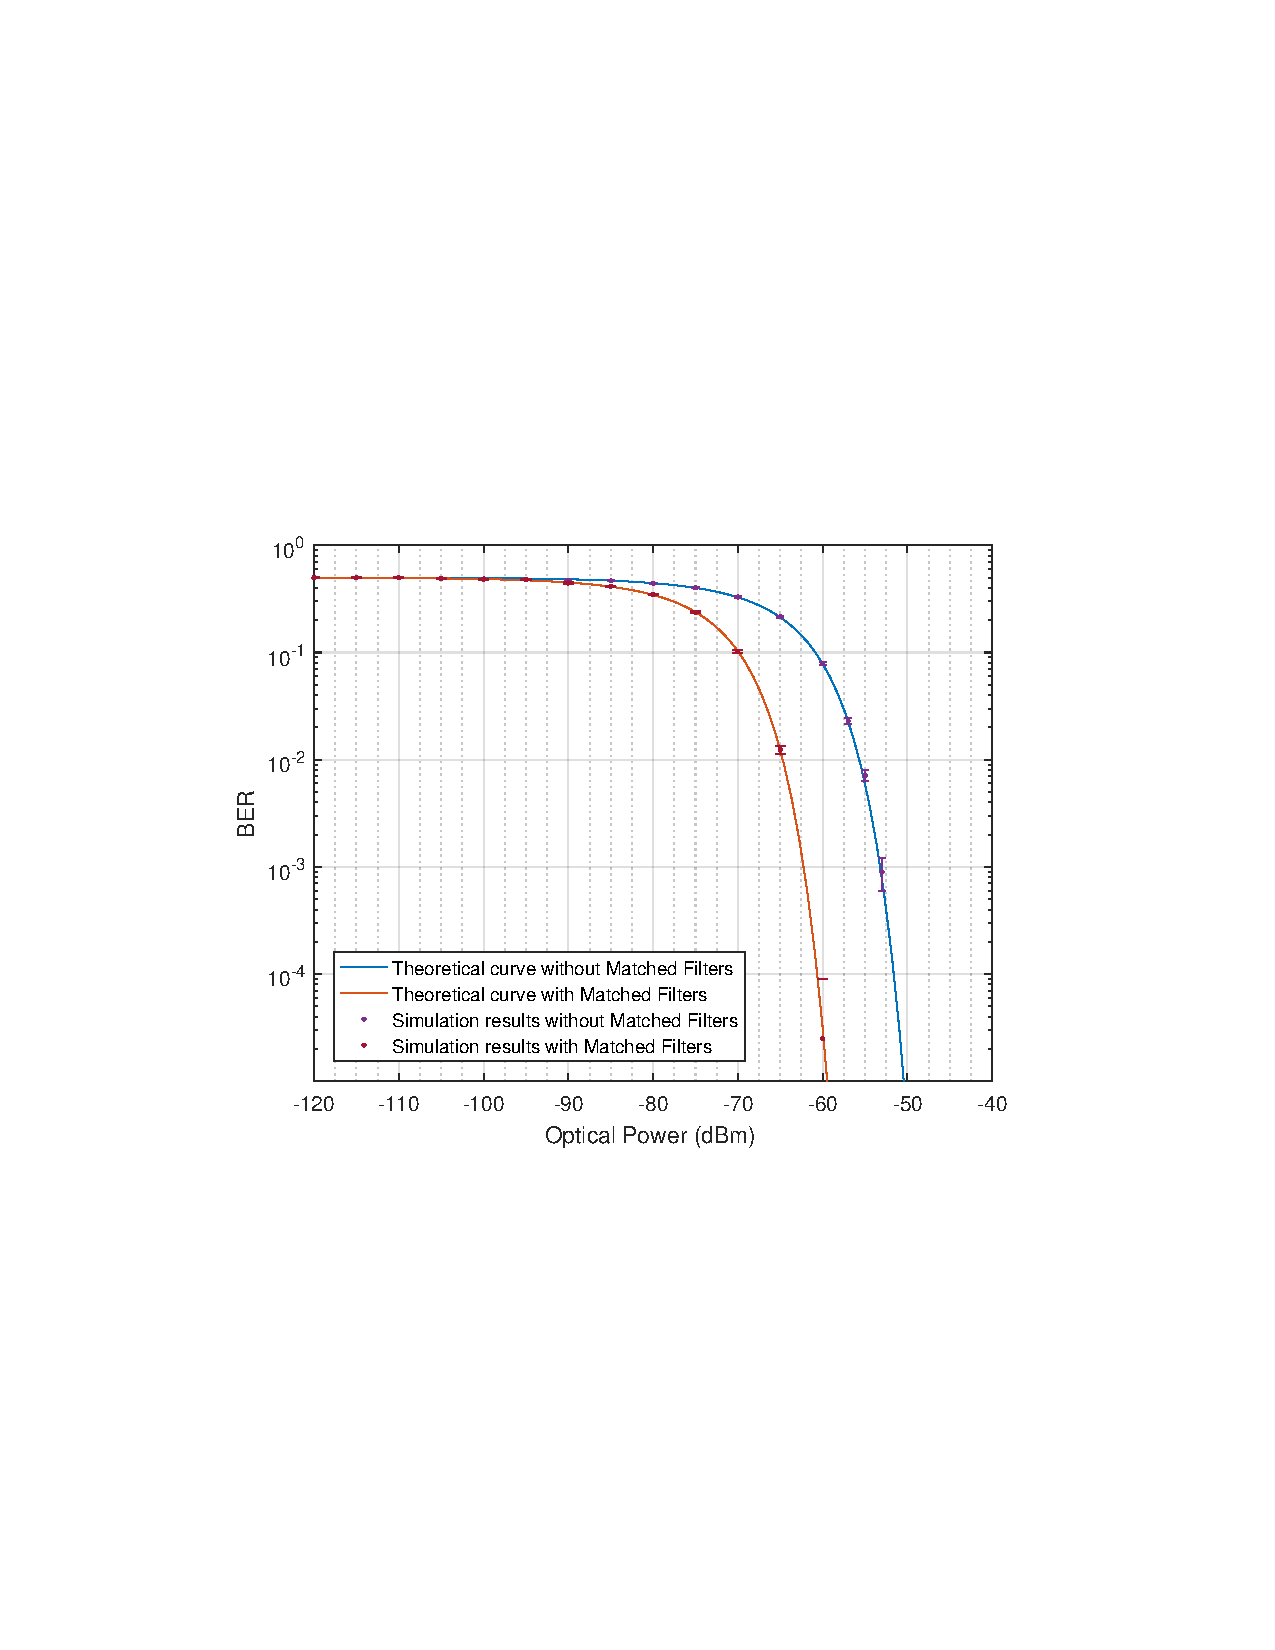
\includegraphics[clip, trim=4cm 8cm 4cm 8cm, width=0.7\textwidth]{./sdf/m_qam_system/figures/teor_vs_simul.pdf}
	\caption{Simulation results for a random binary sequence with $40000$ bits, a noise power of $10^{-6}$ and an amplification of $10^3$. The simulated values which used a matched filter were obtained by shaping the pulse with a root-raised-cosine FIR filter and filtering the signal before the sample with the same filter.}
	\label{fig:ber_pseudorandom}
\end{figure}% 

%\begin{figure}[h]
%	\centering
%	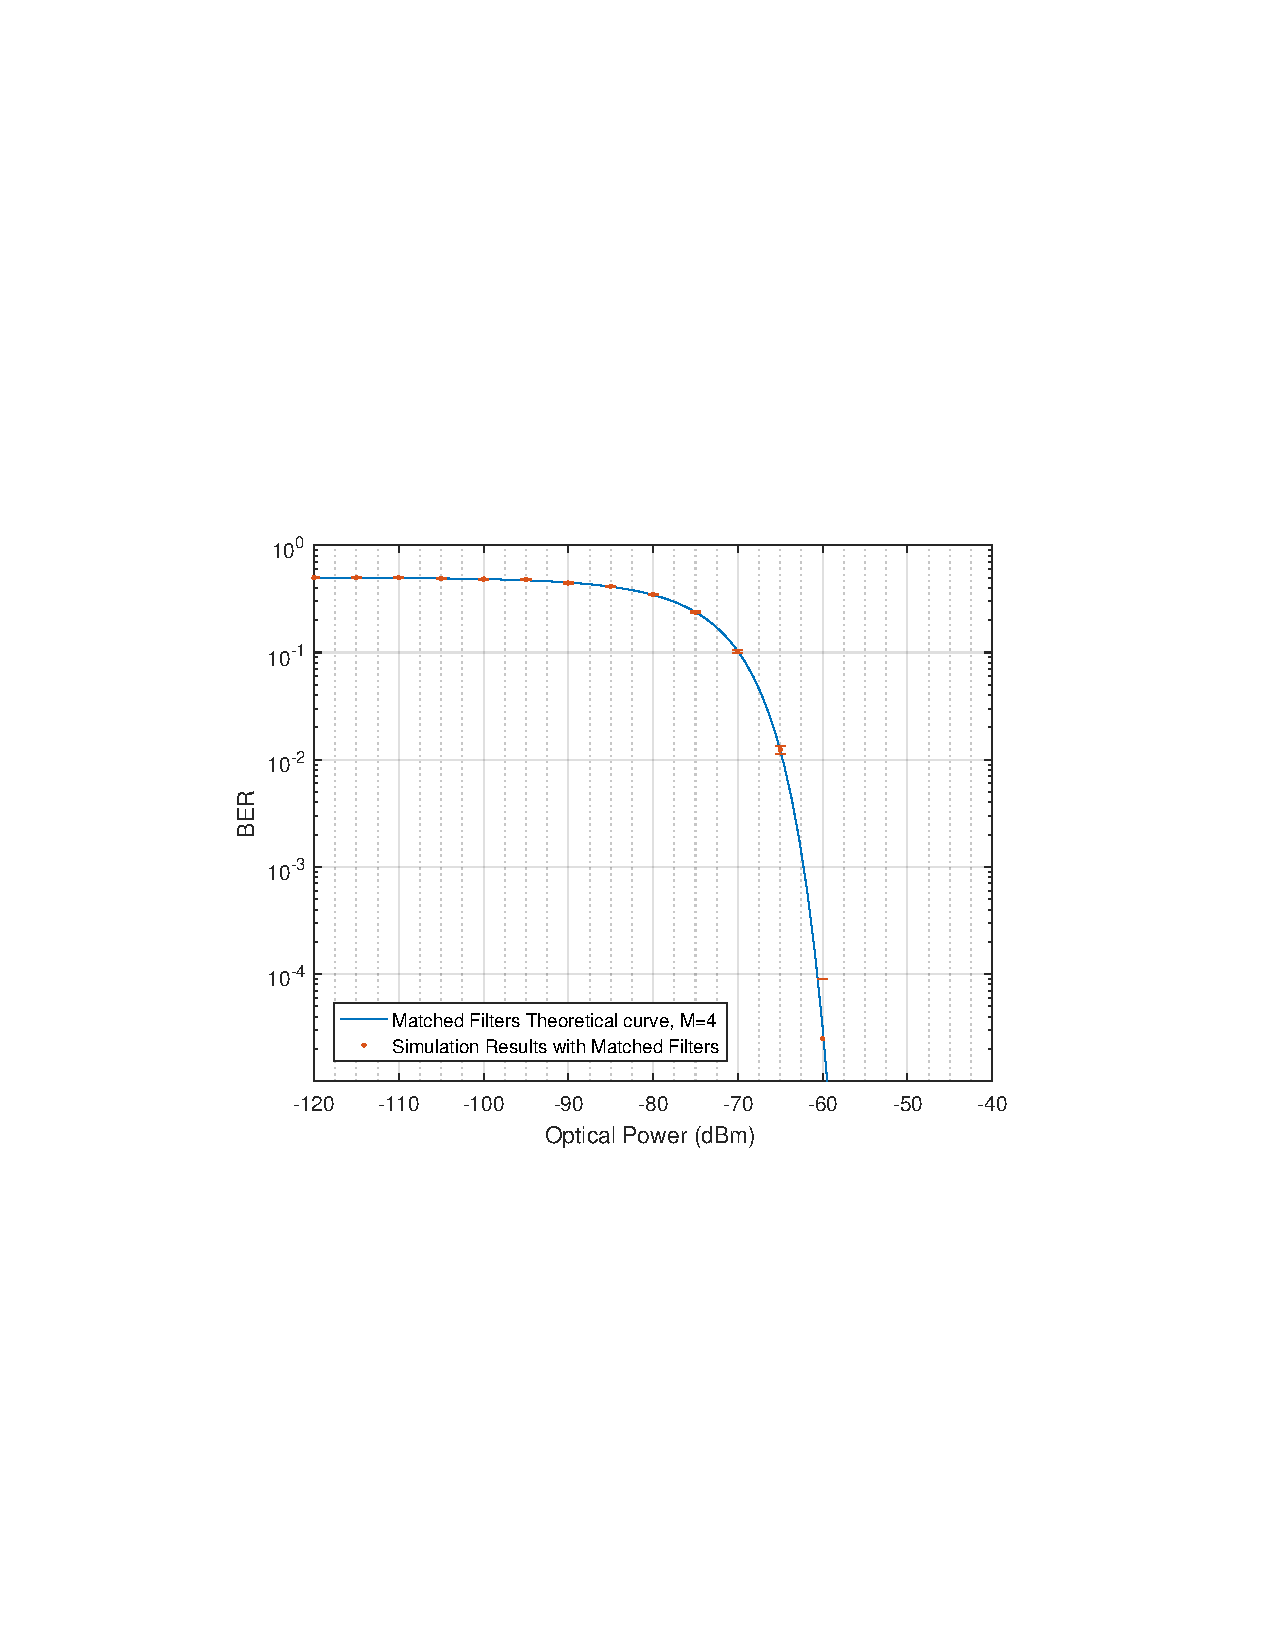
\includegraphics[clip, trim=4cm 8cm 4cm 8cm, width=0.7\textwidth]{./sdf/m_qam_system/figures/BER_QPSK_sim_mf_20180205.pdf}
%	\caption{Simulation result using root-raised cosine matched filtering for a random binary sequence with $40000$ bits, a noise power of $10^{-6}$ and an amplification of $10^3$.}
%	\label{fig:ber_pseudorandom_mf}
%\end{figure}% 


\subsection{Open Issues}

\newpage


%%%%%%%%%%%%%%%%%%%%%%%%%%%%%%%%%%%%%%%%%%%%%%%%%%%%%%%%%%%%%%%%%%%%%%%%%%%%%%%%%%%%%%%%%%%%%%%%%%%%%%%%%%%%
% References
%%%%%%%%%%%%%%%%%%%%%%%%%%%%%%%%%%%%%%%%%%%%%%%%%%%%%%%%%%%%%%%%%%%%%%%%%%%%%%%%%%%%%%%%%%%%%%%%%%%%%%%%%%%%

\renewcommand{\bibname}{References}
%
\bibliographystyle{myIEEEtran}
% argument is your BibTeX string definitions and bibliography database(s)
\bibliography{./sdf/m_qam_system/m_qam_system}
%
%


\cleardoublepage
